\begin{chapterenv}

\chapter{Essential Math Toolkit}

Before we dive into AI and reinforcement learning, let us make sure that we are comfortable with the mathematical language we will be using. Think of this chapter as your toolkit: we are going to explain every symbol, every operation, and every concept that you will see in this book.

\begin{infobox}
\textbf{Don't worry if you're not a math expert!} We'll start from the basics and build up slowly. By the end of this chapter, you'll be comfortable with probability and what it really means, the mysterious ``given'' symbol $|$, why logarithms are so useful, what ``expected value'' means, and how to read mathematical notation.

\textbf{Key promise:} Every single symbol you see later in the book will make sense because we'll explain it here first!
\end{infobox}

\section{Probability: The Language of Uncertainty}

\subsection{What Is Probability?}

\textbf{Probability} is just a fancy way of measuring ``how likely is something to happen?'' We use numbers between 0 and 1:

\begin{itemize}[nosep]
    \item 0 = Impossible (will never happen)
    \item 0.5 = Maybe (50/50 chance)
    \item 1 = Certain (will definitely happen)
\end{itemize}

You can also think of it as percentages: 0 corresponds to 0\%, 0.5 to 50\%, and 1 to 100\%.

\textbf{Notation:} We write $P(\text{event})$ to mean ``the probability of this event happening.''

\paragraph{Example: Coin Flip}

\textbf{Question:} What is the probability of getting heads when you flip a fair coin?

\textbf{Answer:}
\begin{align*}
P(\text{heads}) &= 0.5 = 50\% \\
P(\text{tails}) &= 0.5 = 50\%
\end{align*}

\textbf{Why?} Because the coin has 2 equally likely outcomes and heads are 1 of them, so: $\frac{1}{2} = 0.5$.

\paragraph{Example: Rolling a Die}

\textbf{Question:} What is the probability of rolling a 6 on a fair die?

\textbf{Answer:}
\begin{align*}
P(\text{rolling a 6}) &= \frac{1}{6} \approx 0.167 = 16.7\%
\end{align*}

\textbf{Why?} Because the die has 6 equally likely outcomes (1, 2, 3, 4, 5, 6), and we want just 1 of them (the 6).

\subsection{The ``Given'' Symbol: $|$}

\begin{tipbox}
The vertical bar $|$ is one of the most important symbols you'll see in this book!
\end{tipbox}

$P(A | B)$ is pronounced ``probability of A \textit{given} B.'' It means: ``What is the probability of A happening, \textit{if we already know} that B happened?'' This is called \textbf{conditional probability} because we are computing probability under a certain condition.

Think of the $|$ symbol as a ``knowledge divider'':

\[P(\text{What we want to know} \,|\, \text{What we already know})\]

Everything \textbf{before} $|$ is what we are trying to predict. Everything \textbf{after} $|$ is the information we have.

\paragraph{Example: Weather and Umbrella}

\textbf{Scenario:} You see someone carrying an umbrella.

\textbf{Question 1:} What is the probability that it is raining?
\[P(\text{raining}) = 0.3 \text{ (30\% of days are rainy)}\]

\textbf{Question 2:} What is the probability that it is raining, \textit{given} that you see someone with an umbrella?
\[P(\text{raining} \,|\, \text{umbrella}) = 0.8 \text{ (80\%, much higher!)}\]

\textbf{Why the difference?}
\begin{itemize}[nosep]
    \item Without any information: rain is moderately likely (30\%)
    \item \textit{Given} that you see an umbrella: rain is very likely (80\%)
    \item The umbrella gives us additional information that changes our belief!
\end{itemize}

\paragraph{Example: Language Model Context}

\textbf{For language models, this is EVERYTHING!}

$P(\text{next word} \,|\, \text{all previous words})$

This reads: ``Probability of the next word, \textit{given} all the words we have seen so far.''

\textbf{Example sentence:} ``The cat sat on the \_ \_ \_''.

\begin{align*}
P(\text{``mat''} \,|\, \text{``The cat sat on the''}) &= 0.35 \text{ (35\% likely)} \\
P(\text{``floor''} \,|\, \text{``The cat sat on the''}) &= 0.25 \text{ (25\% likely)} \\
P(\text{``moon''} \,|\, \text{``The cat sat on the''}) &= 0.001 \text{ (very unlikely!)}
\end{align*}

The model uses the context (everything before $|$) to predict what comes next!

\begin{infobox}
\textbf{Practice reading the $|$ symbol:}

\begin{center}
\begin{tabular}{ll}
\toprule
\textbf{Notation} & \textbf{Read as\ldots} \\
\midrule
$P(A | B)$ & ``Probability of A given B'' \\
$P(y | x)$ & ``Probability of y given x'' \\
$P(w_{\text{next}} | w_1, w_2, w_3)$ & ``Probability of next word given words 1, 2, and 3'' \\
$\pi(a | s)$ & ``Probability of action a given state s'' \\
\end{tabular}
\end{center}

\textbf{The key idea:} Everything after the $|$ is ``what we know'' and helps us predict what's before the $|$!
\end{infobox}

\section{Logarithms: Turning Multiplication into Addition}

\subsection{What Is a Logarithm?}

A \textbf{logarithm} (written as $\log$) is the inverse of exponential growth. Think of it this way:

\begin{itemize}[nosep]
    \item \textbf{Exponential:} $2^3 = 8$ means ``2 multiplied by itself 3 times equals 8''
    \item \textbf{Logarithm:} $\log_2(8) = 3$ means ``to what power do I raise 2 to get 8?''
\end{itemize}

\textbf{In this book, $\log$ always means the \textit{natural logarithm}} (base $e \approx 2.718$), also written as $\ln$.

\begin{infobox}
\textbf{Properties of logarithms (these are super useful!):}

\begin{enumerate}[nosep]
    \item \textbf{Log of 1 is always 0:} $\log(1) = 0$. Why? Because $e^0 = 1$.

    \item \textbf{Log of a product = sum of logs:}
    \[\log(A \times B) = \log(A) + \log(B)\]
    This turns multiplication into addition (easier!).

    \item \textbf{Log of a quotient = difference of logs:}
    \[\log\left(\frac{A}{B}\right) = \log(A) - \log(B)\]

    \item \textbf{Log of a power:}
    \[\log(A^n) = n \cdot \log(A)\]
\end{enumerate}

\textbf{Key values to remember:}

\begin{center}
\begin{tabular}{ll}
\toprule
\textbf{Expression} & \textbf{Value} \\
\midrule
$\log(1)$ & $0$ \\
$\log(e)$ & $1$ (where $e \approx 2.718$) \\
$\log(0.5)$ & $\approx -0.693$ (negative because $0.5 < 1$) \\
$\log(2)$ & $\approx 0.693$ \\
$\log(10)$ & $\approx 2.303$ \\
\bottomrule
\end{tabular}
\end{center}
\end{infobox}

\subsection{Why Do We Use Logarithms?}

\textbf{Reason 1: Probabilities multiply, logs add.} When we have multiple independent events:
\[P(\text{both}) = P(\text{event 1}) \times P(\text{event 2})\]

But multiplication with tiny numbers (like $0.0001 \times 0.0001$) gets messy. Logarithms turn this into addition:
\[\log P(\text{both}) = \log P(\text{event 1}) + \log P(\text{event 2})\]

\textbf{Reason 2: Measures ``surprise.''} The logarithm of a probability measures how ``surprising'' an event is:

\begin{itemize}[nosep]
    \item High probability (0.9) $\to$ Low surprise $\to$ $\log(0.9) = -0.105$ (small negative)
    \item Medium probability (0.5) $\to$ Medium surprise $\to$ $\log(0.5) = -0.693$
    \item Low probability (0.1) $\to$ High surprise $\to$ $\log(0.1) = -2.303$ (large negative)
\end{itemize}

We use $-\log$ to flip it so higher surprise = higher value.

\textbf{Reason 3: Numerical stability.} Computers can handle addition better than multiplication of very small numbers. Logs prevent numerical underflow.

\paragraph{Example: Log Probability for a Sentence}

\textbf{Sentence:} ``The cat sat'' (3 words)

\textbf{Probabilities:}
\begin{align*}
P(\text{``The''}) &= 0.4 \\
P(\text{``cat''} \,|\, \text{``The''}) &= 0.3 \\
P(\text{``sat''} \,|\, \text{``The cat''}) &= 0.5
\end{align*}

\textbf{Method 1: Direct multiplication}
\begin{align*}
P(\text{sentence}) &= 0.4 \times 0.3 \times 0.5 = 0.06
\end{align*}

\textbf{Method 2: Log probabilities (better!)}
\begin{align*}
\log P(\text{sentence}) &= \log(0.4) + \log(0.3) + \log(0.5) \\
&= -0.916 + (-1.204) + (-0.693) = -2.813
\end{align*}

Both give the same answer, but Method 2 avoids very small numbers, uses addition (faster for computers), and measures total ``surprise'' of the sentence.

\section{Expected Value: The Average Outcome}

\subsection{What Is Expected Value?}

\textbf{Expected value} (written as $\mathbb{E}[\cdot]$ or sometimes just $E[\cdot]$) is the average value you'd get if you repeated something many times.

\textbf{Formula:}
\[\mathbb{E}[X] = \sum_{\text{all outcomes}} P(\text{outcome}) \times \text{value of outcome}\]

Think of it as: ``If I did this 1000 times, what would my average result be?''

\paragraph{Example: Dice Roll Expected Value}

\textbf{Question:} What's the expected value when rolling a fair die?

\textbf{Answer:}
\begin{align*}
\mathbb{E}[\text{die}] &= P(1) \times 1 + P(2) \times 2 + P(3) \times 3 + P(4) \times 4 + P(5) \times 5 + P(6) \times 6 \\
&= \frac{1}{6} \times 1 + \frac{1}{6} \times 2 + \frac{1}{6} \times 3 + \frac{1}{6} \times 4 + \frac{1}{6} \times 5 + \frac{1}{6} \times 6 \\
&= \frac{1 + 2 + 3 + 4 + 5 + 6}{6} = \frac{21}{6} = 3.5
\end{align*}

\textbf{Interpretation:} If you roll the die many times, your average result will be 3.5! (You can never roll 3.5 on a single roll, but the average over many rolls is 3.5.)

\paragraph{Example: Reward in Reinforcement Learning}

\textbf{Scenario:} An AI generates responses and gets rewards:

\begin{center}
\begin{tabular}{lcc}
\toprule
\textbf{Response quality} & \textbf{Probability} & \textbf{Reward} \\
\midrule
Excellent & 20\% & +10 \\
Good & 50\% & +5 \\
Mediocre & 25\% & 0 \\
Bad & 5\% & $-5$ \\
\bottomrule
\end{tabular}
\end{center}

\textbf{Expected reward:}
\begin{align*}
\mathbb{E}[\text{reward}] &= 0.20 \times 10 + 0.50 \times 5 + 0.25 \times 0 + 0.05 \times (-5) \\
&= 2 + 2.5 + 0 - 0.25 = 4.25
\end{align*}

\textbf{Meaning:} On average, this AI gets +4.25 reward per response. The goal of training is to increase this expected value!

\subsection{Expected Value with Conditions}

\begin{infobox}
\textbf{Conditional Expected Value}

\begin{center}
\begin{tabular}{p{0.43\textwidth}p{0.43\textwidth}}
\toprule
\textbf{Formal Math} & \textbf{What It Really Means} \\
\midrule
$\mathbb{E}_{X \sim P}[f(X)]$ & Expected value of function $f$ when $X$ follows distribution $P$ \\
\midrule
$\mathbb{E}[\cdot]$ & Expected value (average) \\
$X \sim P$ & Variable $X$ is drawn from distribution $P$ \\
$f(X)$ & We're averaging the values of $f(X)$, not $X$ itself \\
\bottomrule
\end{tabular}
\end{center}
\end{infobox}

\paragraph{Example: Language Model Expected Loss}

When training a language model:

\[\mathbb{E}_{(x,y) \sim \mathcal{D}}[\text{loss}(x,y)]\]

This reads as: ``Expected loss when we sample prompt-response pairs $(x,y)$ from our dataset $\mathcal{D}$.''

\textbf{In plain English:} ``Average loss across all examples in our training data.''

\section{Summation Notation: Adding Things Up}

\subsection{The $\sum$ Symbol}

The symbol $\sum$ (capital Greek letter sigma) means ``add up all of these things.''

\textbf{Basic form:}
\[\sum_{i=1}^{n} x_i = x_1 + x_2 + x_3 + \cdots + x_n\]

\textbf{Reading:} ``Sum from $i$ equals 1 to $n$ of $x_i$.'' The letter $i$ is the \textbf{index} that counts from the starting value (1) to the ending value ($n$).

\paragraph{Example: Simple Sum}

\[\sum_{i=1}^{5} i = 1 + 2 + 3 + 4 + 5 = 15\]

\[\sum_{i=1}^{4} 2i = 2(1) + 2(2) + 2(3) + 2(4) = 2 + 4 + 6 + 8 = 20\]

\paragraph{Example: Sum in Machine Learning}

\textbf{Computing loss for a sequence:}

\[\text{Total loss} = \sum_{t=1}^{T} \ell_t\]

This means: ``Add up the loss at each time step from $t=1$ to $t=T$.''

If $T=4$ and losses are: $\ell_1 = 0.5$, $\ell_2 = 0.3$, $\ell_3 = 0.8$, $\ell_4 = 0.4$:

\[\sum_{t=1}^{4} \ell_t = 0.5 + 0.3 + 0.8 + 0.4 = 2.0\]

\subsection{Infinity in Summation}

Sometimes we sum ``forever'':

\[\sum_{t=0}^{\infty} r_t\]

This means: ``Add up all rewards from time 0 to infinity.''

\begin{infobox}
\textbf{Don't panic!} In practice, we use a \textit{discount factor} that makes future terms tiny, or we stop after a finite number of steps, or the series converges to a finite value.
\end{infobox}

\section{Functions and Notation}

\subsection{Functions as Black Boxes}

A \textbf{function} is like a machine: you put something in (the input), it does some computation, and you get something out (the output).

\textbf{Notation:} $f(x)$ means ``function $f$ applied to input $x$.''

\textbf{Example functions:}
\begin{itemize}[nosep]
    \item $f(x) = 2x$: doubles the input
    \item $g(x) = x^2$: squares the input
    \item $h(x) = \log(x)$: takes the log of the input
\end{itemize}

\subsection{The Sigmoid Function}

\begin{infobox}
\textbf{The Sigmoid Function $\sigma$}

\begin{center}
\begin{tabular}{p{0.43\textwidth}p{0.43\textwidth}}
\toprule
\textbf{Formal Math} & \textbf{What It Really Means} \\
\midrule
$\sigma(z) = \frac{1}{1 + e^{-z}}$ & Squash any number to range [0, 1] \\
\midrule
$\sigma(0) = 0.5$ & Zero input gives 50\% output \\
$\sigma(+\infty) = 1$ & Very large positive input $\to$ 1 \\
$\sigma(-\infty) = 0$ & Very large negative input $\to$ 0 \\
\bottomrule
\end{tabular}
\end{center}
\end{infobox}

\textbf{Sigmoid in action:}

\begin{center}
\begin{tabular}{ccc}
\toprule
\textbf{Input $z$} & \textbf{$\sigma(z)$} & \textbf{As percentage} \\
\midrule
$-5$ & 0.007 & 0.7\% \\
$-3$ & 0.047 & 4.7\% \\
$-1$ & 0.269 & 26.9\% \\
$0$ & 0.500 & 50.0\% \\
$+1$ & 0.731 & 73.1\% \\
$+3$ & 0.953 & 95.3\% \\
$+5$ & 0.993 & 99.3\% \\
\bottomrule
\end{tabular}
\end{center}

\textbf{Why it is useful:} The sigmoid converts any real number to a probability, it is smooth and differentiable (good for training), and it is used everywhere in neural networks and RL!

\section{Loss Functions: Measuring Mistakes}

\subsection{What Is a Loss Function?}

A \textbf{loss function} (written as $\mathcal{L}$ or $L$) measures ``how wrong'' our model is. The key idea: lower loss means better model, and higher loss means worse model. Training a model means finding parameters that \textit{minimize} the loss.

\begin{tipbox}
Think of loss like a golf score; your score should be as low as possible, and each mistake increases it.
\end{tipbox}

\subsection{Common Loss Functions}

\begin{infobox}
\textbf{Negative Log Likelihood Loss}

\begin{center}
\begin{tabular}{p{0.43\textwidth}p{0.43\textwidth}}
\toprule
\textbf{Formal Math} & \textbf{What It Really Means} \\
\midrule
$\mathcal{L} = -\log P(\text{correct})$ & Loss = Negative log probability of correct answer \\
\bottomrule
\end{tabular}
\end{center}

\textbf{Why this makes sense:}
\begin{itemize}[nosep]
    \item If model is confident in correct answer ($P = 0.99$), loss is small ($-\log(0.99) = 0.01$).
    \item If model is unsure ($P = 0.5$), loss is larger ($-\log(0.5) = 0.69$).
    \item If model is wrong ($P = 0.01$), loss is huge ($-\log(0.01) = 4.6$).
\end{itemize}
\end{infobox}

\paragraph{Example: Loss for Word Prediction}

Model predicts next word probabilities:

\begin{center}
\begin{tabular}{lcc}
\toprule
\textbf{Word} & \textbf{Probability} & \textbf{Loss if correct} \\
\midrule
``cat'' & 0.8 & $-\log(0.8) = 0.22$ (good!) \\
``dog'' & 0.15 & $-\log(0.15) = 1.90$ (okay) \\
``airplane'' & 0.01 & $-\log(0.01) = 4.61$ (bad!) \\
\bottomrule
\end{tabular}
\end{center}

\textbf{If the correct word was ``cat'':} Loss = 0.22. \textbf{and if the correct word was ``airplane'':} Loss = 4.61 (model was very wrong!). Training adjusts the model to reduce these losses.

\section{Gradients and Optimization}

\subsection{What Is a Gradient?}

A \textbf{gradient} tells you which direction to go in to reduce the loss.

\textbf{Analogy:} Imagine that you are on a foggy mountain trying to get to the lowest point (valley). The gradient tells you which direction is ``downhill,'' you take a small step in that direction, and repeat until you reach the bottom. This process is called \textbf{gradient descent}.

\textbf{In machine learning:}
\begin{itemize}[nosep]
    \item The ``mountain'' is the loss function
    \item The ``location'' is your model parameters
    \item The ``valley'' is the best parameters (minimum loss)
\end{itemize}

\subsection{The Training Loop}

\begin{infobox}
\textbf{How gradient descent works:}

\begin{enumerate}[nosep]
    \item \textbf{Start} with random parameters $\theta$
    \item \textbf{Compute loss} $\mathcal{L}(\theta)$ on training data
    \item \textbf{Compute gradient} $\nabla_\theta \mathcal{L}$ (which direction reduces loss?)
    \item \textbf{Update parameters:}
    \[\theta_{\text{new}} = \theta_{\text{old}} - \alpha \cdot \nabla_\theta \mathcal{L}\]
    where $\alpha$ is the \textit{learning rate} (step size)
    \item \textbf{Repeat} steps 2--4 many times
    \item \textbf{Done} when loss stops decreasing
\end{enumerate}

\textbf{The gradient $\nabla_\theta$ just means:} ``How does loss change when I change each parameter?''
\end{infobox}

\section{Notation Reference Card}

The following table summarizes all the mathematical notation used throughout this book. Recall this table whenever you encounter an unfamiliar symbol.

\begin{center}
\begin{tabular}{p{0.2\textwidth}p{0.3\textwidth}p{0.35\textwidth}}
\toprule
\textbf{Symbol} & \textbf{Name} & \textbf{Meaning} \\
\midrule
$P(A)$ & Probability & Chance of event $A$ \\
$P(A | B)$ & Conditional probability & Probability of $A$ given $B$ \\
$|$ & ``Given'' & Separates condition from prediction \\
$\log(x)$ & Logarithm & Inverse of exponential \\
$\mathbb{E}[X]$ & Expected value & Average value of $X$ \\
$\sum_{i=1}^{n}$ & Summation & Add from $i=1$ to $i=n$ \\
$\mathcal{L}$ & Loss function & Measure of model error \\
$\theta$ & Parameters & Model weights (billions of numbers) \\
$\pi$ & Policy & Decision-making strategy \\
$\sigma(z)$ & Sigmoid & Squash to [0,1] range \\
$\nabla$ & Gradient & Direction of steepest increase \\
$\sim$ & ``Drawn from'' & Sample from distribution \\
$\in$ & ``Element of'' & Belongs to a set \\
$\approx$ & Approximately & Roughly equal \\
\bottomrule
\end{tabular}
\end{center}

The visual cheat sheet below brings all of these ideas together in one place -- keep it handy as you work through the rest of the book.

\clearpage
\begin{figure}[!h]
\centering
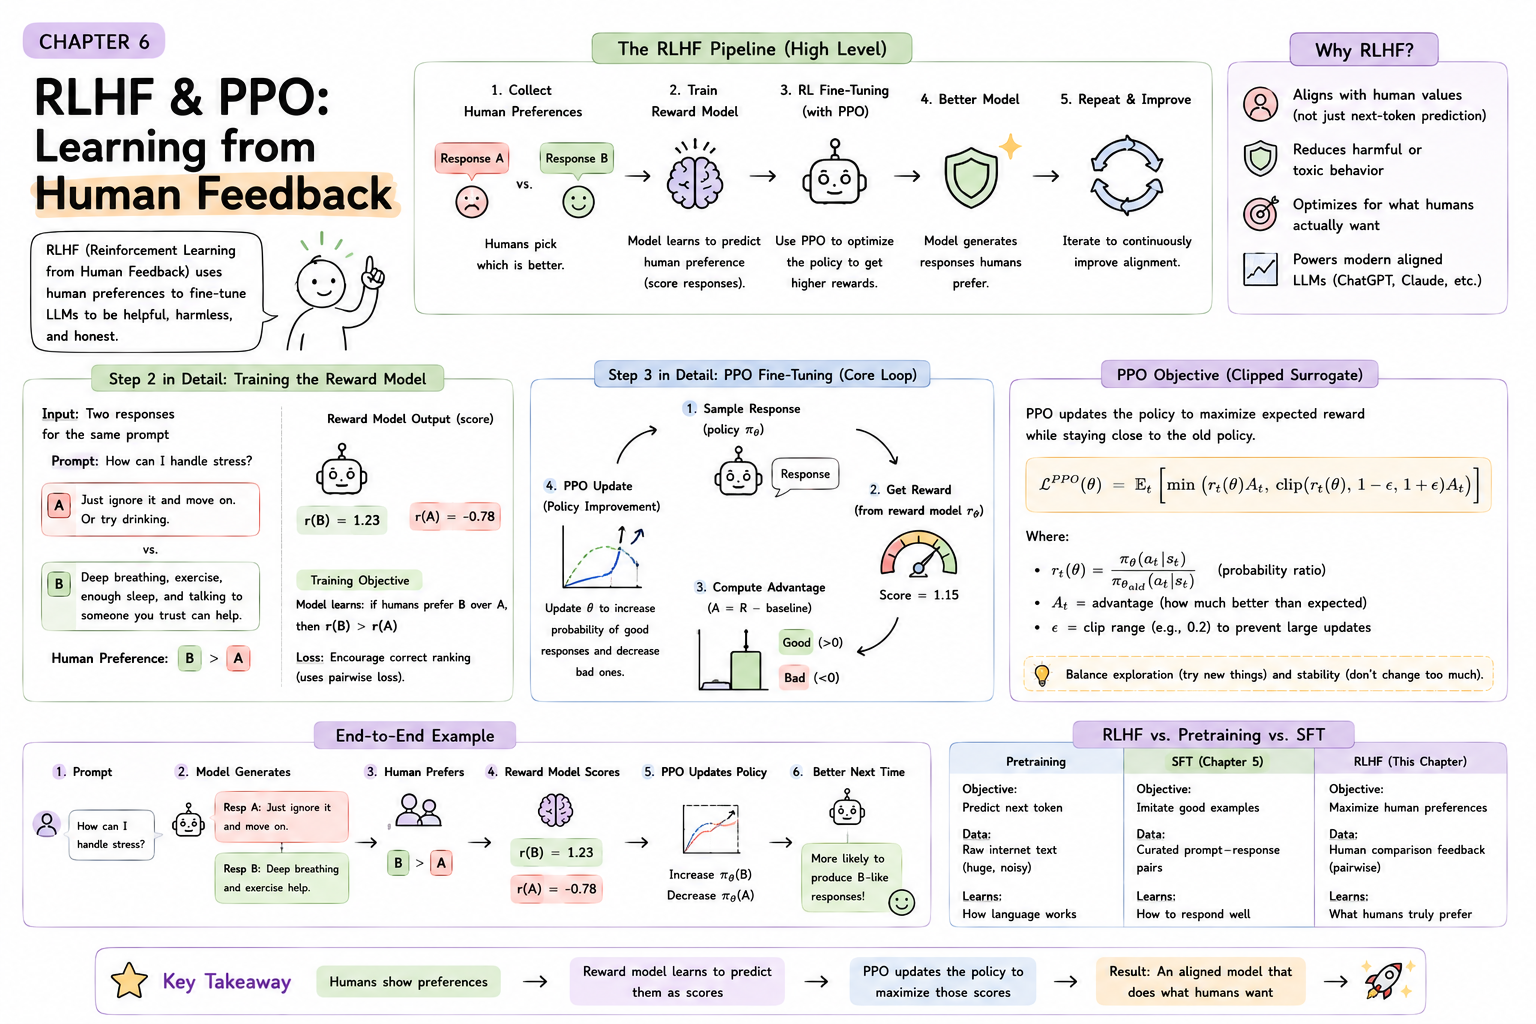
\includegraphics[width=0.88\textwidth]{images/ch01_fig01_math_overview.png}
\caption{Visual cheat sheet -- all Chapter 1 math concepts at a glance.}
\label{fig:ch01:math_overview}
\end{figure}

\begin{infobox}
\textbf{You now have all the mathematical tools you need!}

Every equation in this book uses these concepts. When you see complex formulas later, remember: break them down into pieces, identify the symbols from this chapter, read the plain English explanations, and work through the numerical examples.

\textbf{You're ready for the main content!}
\end{infobox}


\begin{tipbox}
\textbf{Companion notebook.} The code for this chapter is available at:\\[3pt]
\texttt{github.com/arunpshankar/packt-final}\\[3pt]
Swap \texttt{github.com} for \texttt{githubtocolab.com} to open in Colab.
\end{tipbox}

\end{chapterenv}